% Figure s03f03 (Session 3): the SSH chain in its two dimerizations, with the spectra.
% The image is rendered by figures/blender/s03f03_ssh.py; the coordinates of the labels come from
% figures/blender/out/s03f03_ssh_anchors.tex. Build with figures/blender/build_figure.sh s03f03_ssh.
\documentclass[11pt,tikz,border=0pt]{standalone}
\usepackage[T1]{fontenc}
\usepackage{amsmath,amssymb,graphicx}
\usepackage{xcolor}
% The three label colors of the figures, with the same values as in src/figures_preamble.tex.
\definecolor{aqmaccent}{RGB}{31,78,121}
\definecolor{aqmbroken}{RGB}{168,42,34}
\definecolor{aqmmuted}{RGB}{125,125,125}

\newlength{\figw}\setlength{\figw}{17.91cm}   % 1.10 of the text width, before the empty margins of the render are cropped

\begin{document}
\begin{tikzpicture}[lbl/.style={font=\small, inner sep=1.5pt}]
  \node[overlay, anchor=south west, inner sep=0pt] at (0,0)
    {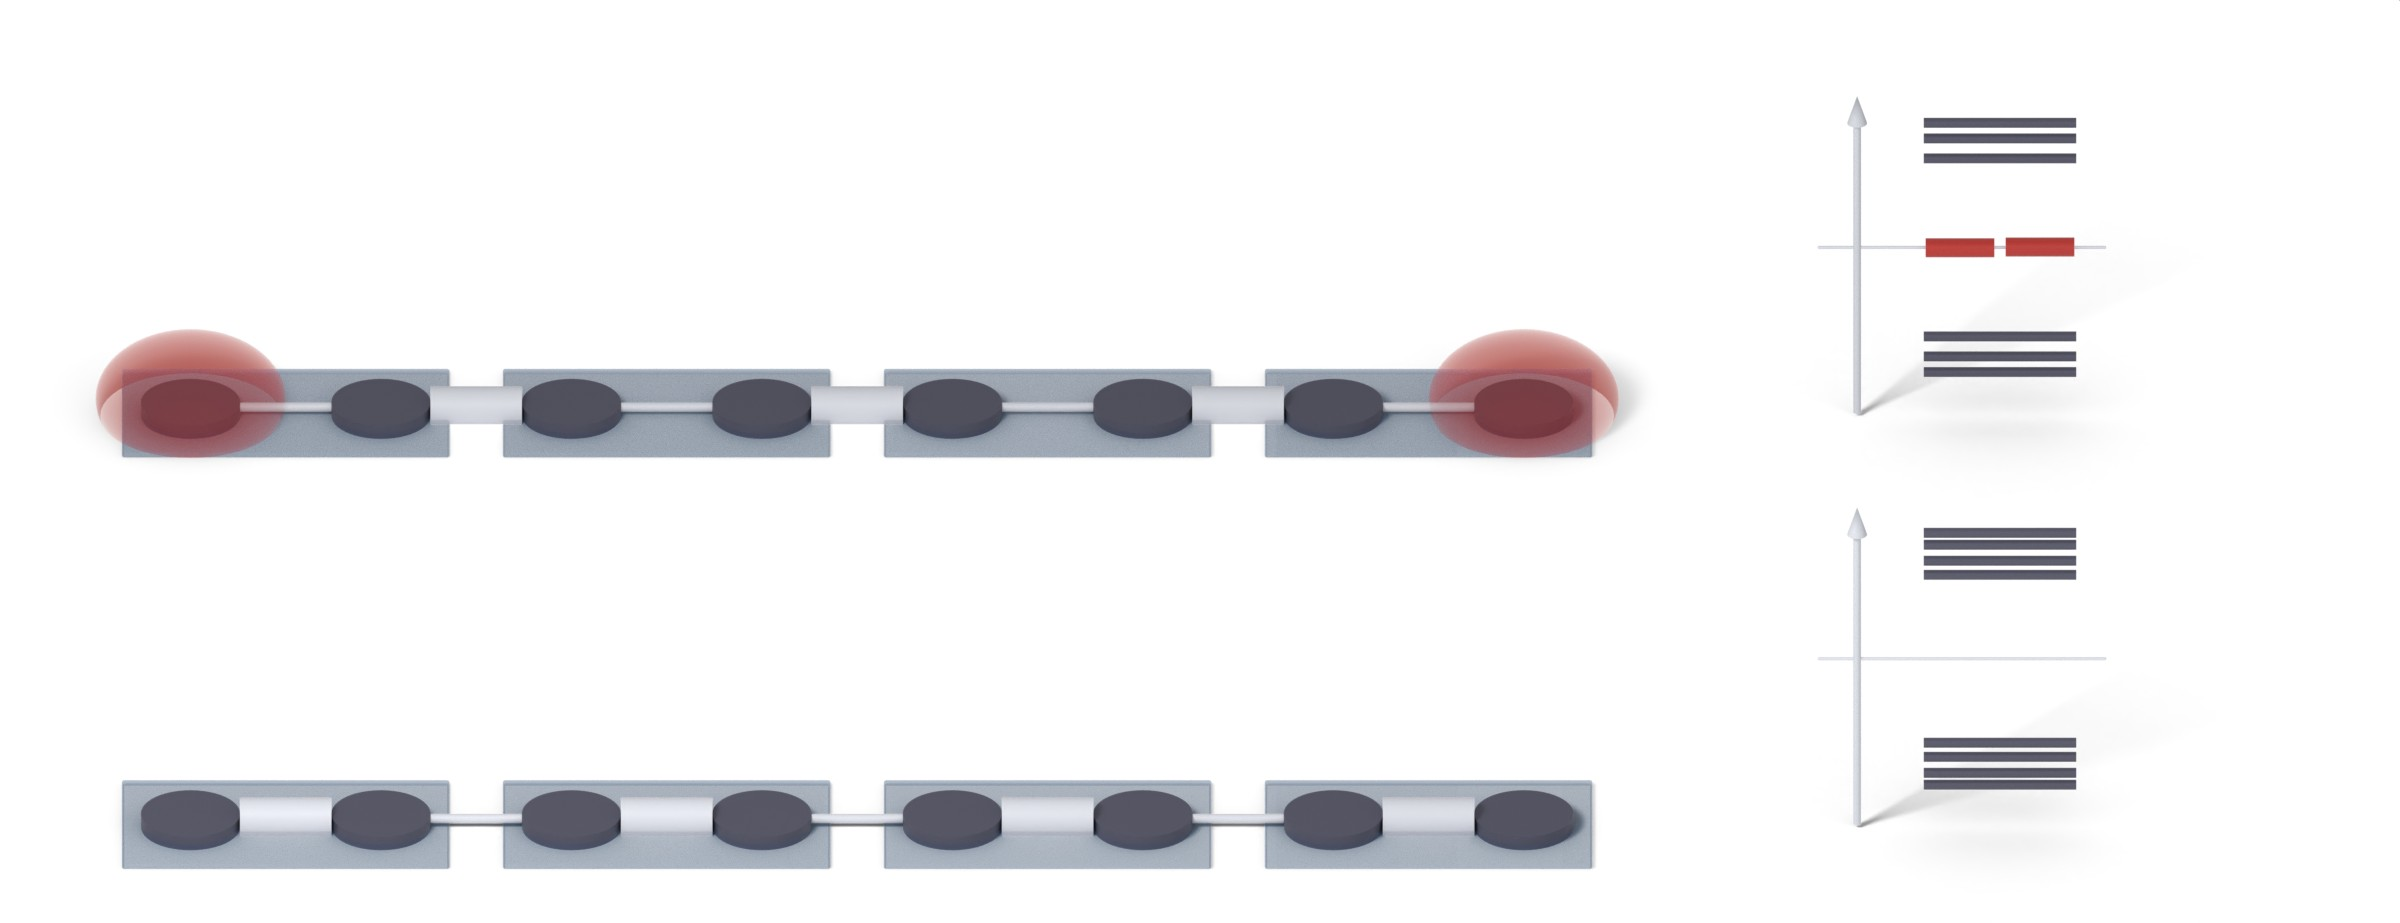
\includegraphics[width=\figw]{../blender/out/s03f03_ssh.jpg}};
  % written by build_figure.sh; the painted part of the image
\path (0.0346\figw,0.0221\figw) rectangle (0.8779\figw,0.3446\figw);

  %% written by figlib.py; x and y in units of the image width
\coordinate (aE) at (0.7738\figw,0.1766\figw);
\coordinate (azero) at (0.7659\figw,0.1101\figw);
\coordinate (atop) at (0.8690\figw,0.1535\figw);
\coordinate (abot) at (0.8690\figw,0.0667\figw);
\coordinate (apanel) at (0.0437\figw,0.1066\figw);
\coordinate (at) at (0.2778\figw,0.0582\figw);
\coordinate (aone) at (0.3571\figw,0.0582\figw);
\coordinate (bE) at (0.7738\figw,0.3480\figw);
\coordinate (bzero) at (0.7659\figw,0.2815\figw);
\coordinate (btop) at (0.8690\figw,0.3249\figw);
\coordinate (bbot) at (0.8690\figw,0.2380\figw);
\coordinate (bpanel) at (0.0437\figw,0.2780\figw);
\coordinate (bendL) at (0.0794\figw,0.2408\figw);
\coordinate (bendR) at (0.6349\figw,0.2408\figw);
\coordinate (bt) at (0.2778\figw,0.2296\figw);
\coordinate (bone) at (0.3571\figw,0.2296\figw);

  % (a) in front: the trivial chain
  \node[lbl, anchor=south west] at (apanel) {\textbf{(a)}\quad intracell hopping dominates, $t\gg1$, trivial};
  \node[lbl, anchor=south] at (at) {$t$};
  \node[lbl, anchor=south] at (aone) {$1$};
  \node[lbl, anchor=south] at (aE) {$E$};
  \node[lbl, anchor=east, text=aqmmuted] at (azero) {$0$};
  \node[lbl, anchor=west] at (atop) {$+t$};
  \node[lbl, anchor=west] at (abot) {$-t$};
  % (b) behind: the topological chain
  \node[lbl, anchor=south west] at (bpanel) {\textbf{(b)}\quad intercell hopping dominates, $t\to0$, topological};
  \node[lbl, anchor=south] at (bt) {$t$};
  \node[lbl, anchor=south] at (bone) {$1$};
  \node[lbl, anchor=south, text=aqmbroken] at (bendL) {end state};
  \node[lbl, anchor=south, text=aqmbroken] at (bendR) {end state};
  \node[lbl, anchor=south] at (bE) {$E$};
  \node[lbl, anchor=east, text=aqmbroken] at (bzero) {$0$};
  \node[lbl, anchor=west] at (btop) {$+1$};
  \node[lbl, anchor=west] at (bbot) {$-1$};
\end{tikzpicture}
\end{document}
